\ieeesection[Software Design: Autonomous Navigation and System Architecture]{Software Design: Autonomous Navigation and System Architecture}
\label{sec:software}

\textcolor{gray}{\rule{\linewidth}{3pt}}


\subsection{Architecture Overview}
\label{sec:arch_overview}

The software subsystem of CourtSweeper is structured as a hierarchical two-layer Finite State Machine (FSM) architecture, as illustrated in Figure~\ref{fig:fsm_overview}. All modules run on the NVIDIA Jetson Orin NX edge computing unit, bridging heterogeneous sensory inputs (DJI camera, RPLidar, IR proximity sensor) with mechanical outputs (Mecanum chassis, dual-roller intake) through a ROS2-based middleware layer.

\begin{figure}[!htb]
  \centering
  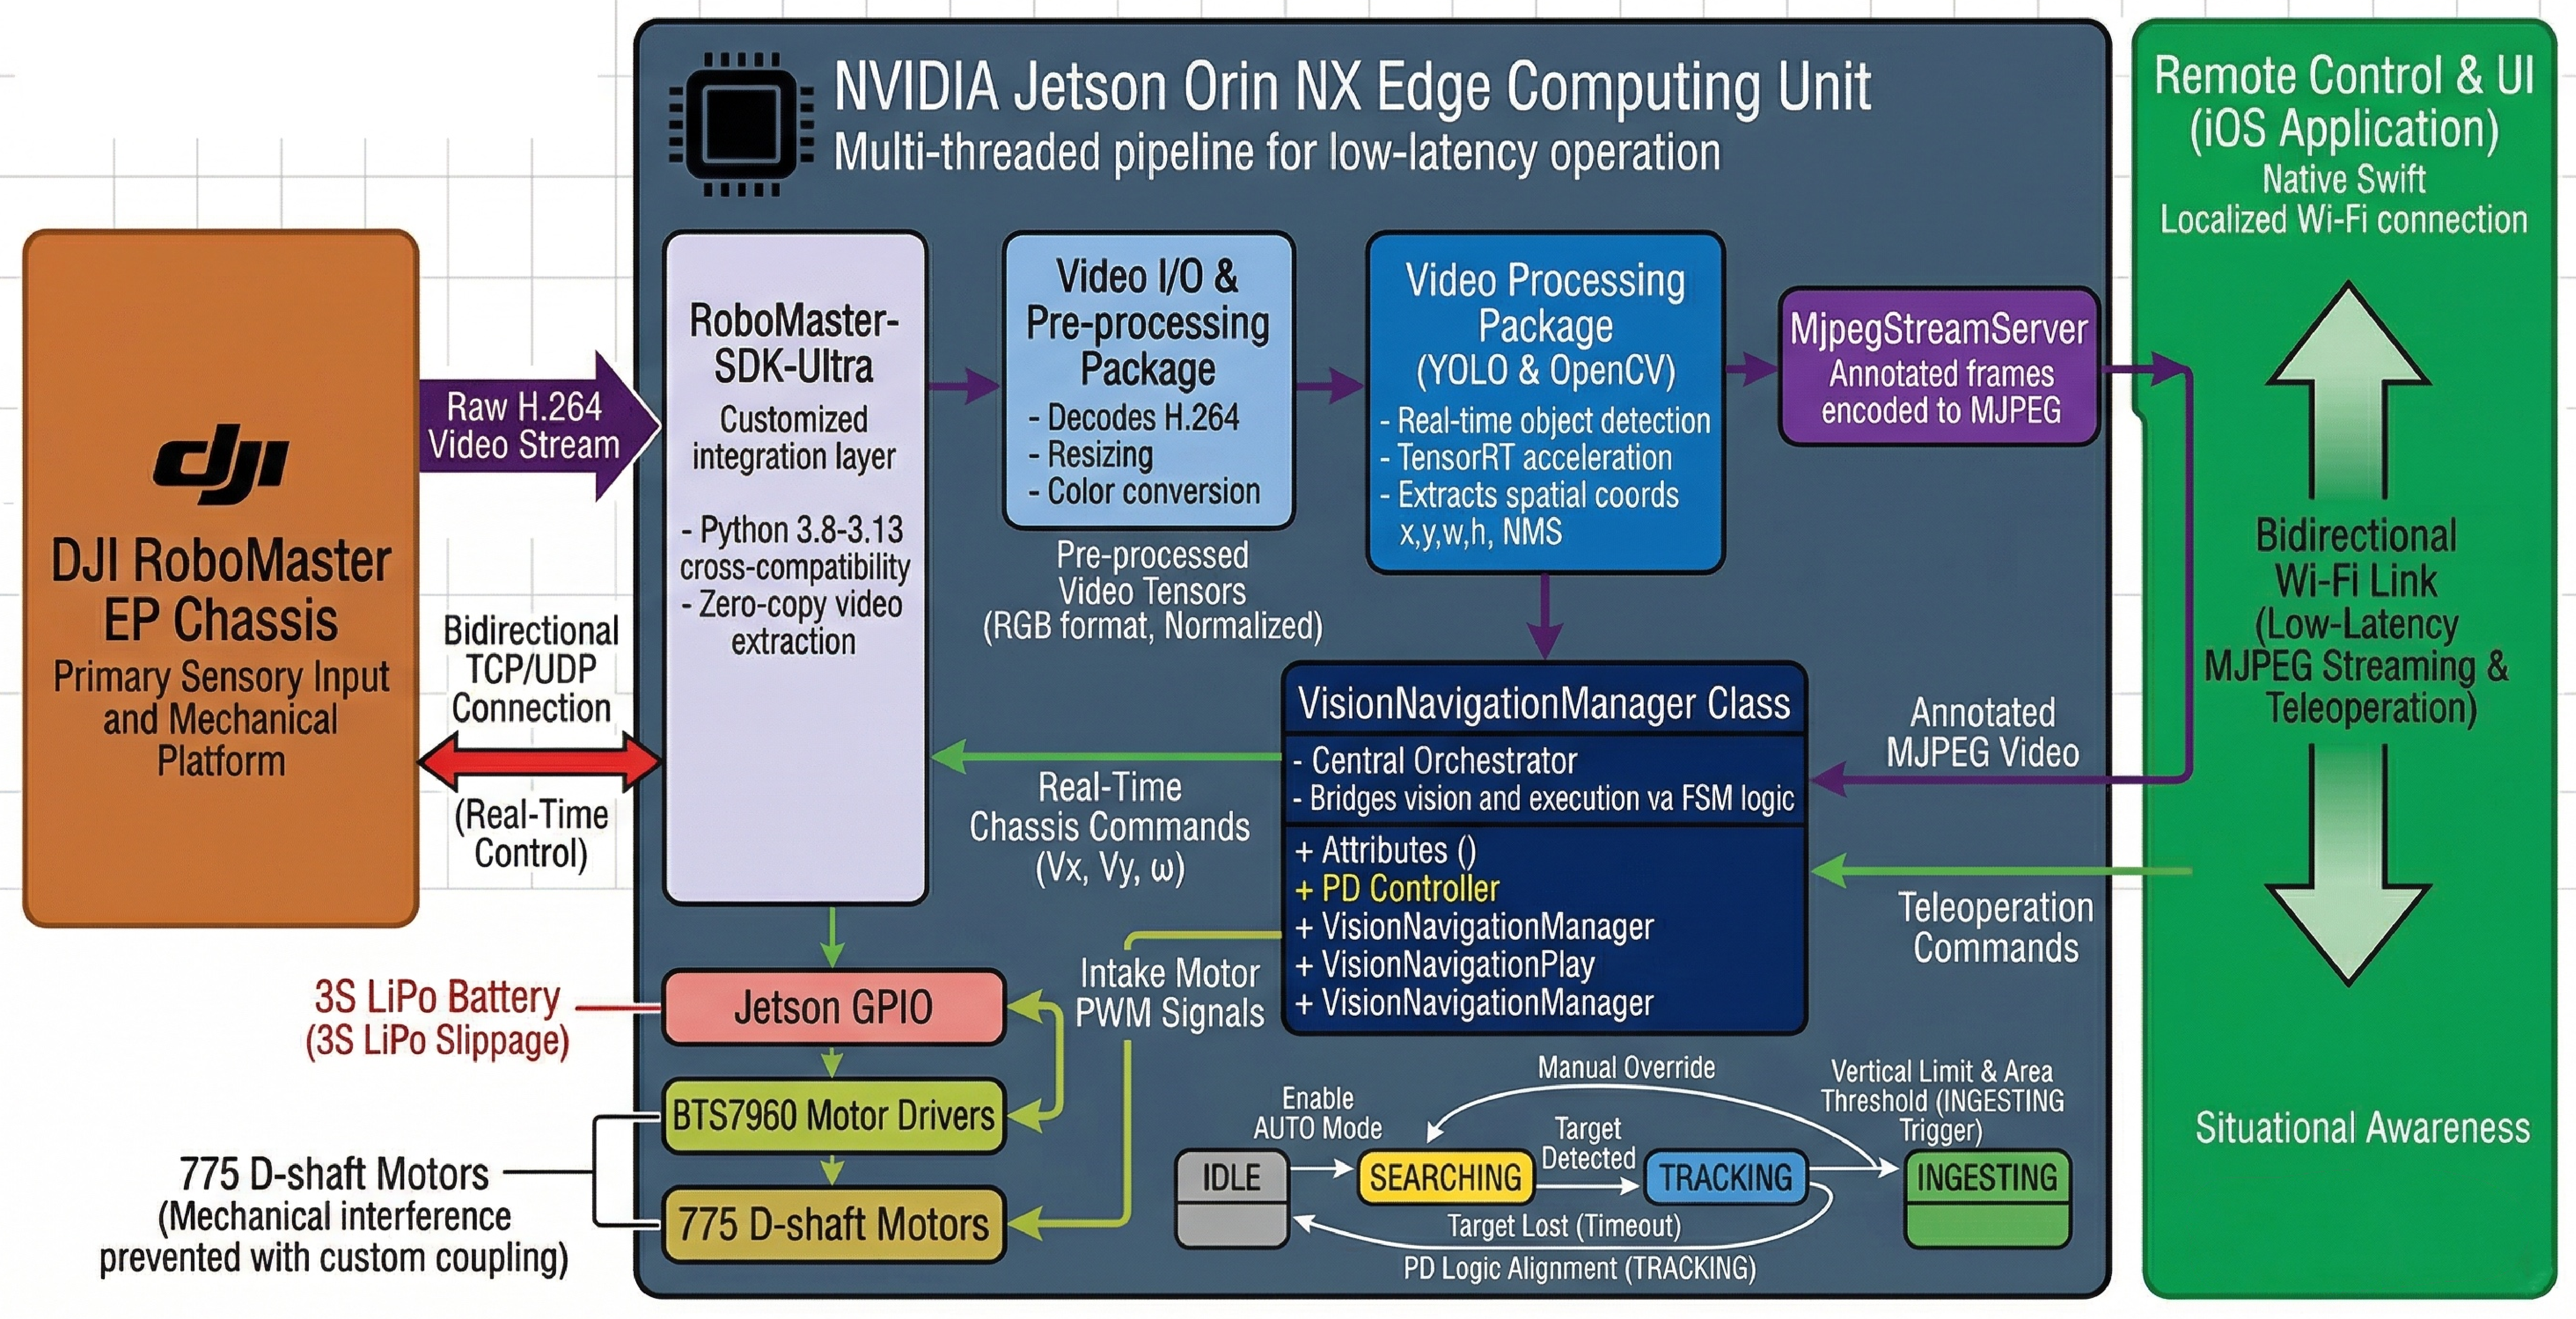
\includegraphics[width=0.95\linewidth]{figures/fig_software_overview.pdf}
  \caption{The hierarchical software architecture of CourtSweeper. The upper layer handles iOS interrupt commands, while the lower layer executes the autonomous workflow through three sequential phases.}
  \label{fig:fsm_overview}
\end{figure}

Every ROS2 bridge node in the system follows a uniform initialization pattern, establishing a 50\,Hz control loop timer and subscribing to the \texttt{/cmd\_vel} topic for navigation command forwarding:

\begin{minted}{python}
class RoboMasterBridge(Node):
    def __init__(self):
        super().__init__('robomaster_bridge')
        self.odom_pub   = self.create_publisher(Odometry, '/odom', 10)
        self.camera_pub = self.create_publisher(CompressedImage,
                            '/camera/image/compressed', 10)
        self.cmd_sub    = self.create_subscription(Twist,
                            '/cmd_vel', self.cmd_vel_callback, 10)
        self.tf_broadcaster = TransformBroadcaster(self)
        self.timer = self.create_timer(0.02, self.timer_callback)
\end{minted}

The critical ROS2 data streams flowing through this middleware layer are summarized in Table~\ref{tab:ros2_topics}.

\begin{table}[!htb]
  \footnotesize
  \centering
  \caption{Core ROS2 topics bridging the DJI chassis and the navigation/vision stacks.}
  \label{tab:ros2_topics}
  \begin{tabular}{@{}llcl@{}}
    \toprule
    \textbf{Topic} & \textbf{Message Type} & \textbf{Rate} & \textbf{Direction} \\
    \midrule
    \texttt{/odom} & \texttt{nav\_msgs/Odometry} & 50\,Hz & Chassis $\to$ ROS2 \\
    \texttt{/camera/image/compressed} & \texttt{sensor\_msgs/CompressedImage} & 10\,Hz & Chassis $\to$ ROS2 \\
    \texttt{/camera/camera\_info} & \texttt{sensor\_msgs/CameraInfo} & 10\,Hz & Chassis $\to$ ROS2 \\
    \texttt{/cmd\_vel} & \texttt{geometry\_msgs/Twist} & On demand & ROS2 $\to$ Chassis \\
    \texttt{/scan} & \texttt{sensor\_msgs/LaserScan} & \textasciitilde10\,Hz & LiDAR $\to$ ROS2 \\
    \texttt{/tf} (odom$\to$base\_footprint) & \texttt{tf2\_msgs/TFMessage} & 50\,Hz & Bridge $\to$ ROS2 \\
    \bottomrule
  \end{tabular}
\end{table}


\subsection{Chassis Navigation \& DJI SDK Integration}
\label{sec:dji-sdk}

To interface with the mobile platform, the system implements \textbf{RoboMaster-SDK-Ultra}, a high-performance community fork of the official DJI Python SDK. The robot connects to the Jetson via Wi-Fi in Station (STA) mode and is set to free-motion mode before any chassis commands are issued:

\begin{minted}{python}
from robomaster_ultra import robot

ep_robot = robot.Robot()
ep_robot.initialize(conn_type="sta")
ep_robot.set_robot_mode(mode="free")
ep_chassis = ep_robot.chassis
\end{minted}

Velocity commands arriving via \texttt{/cmd\_vel} are converted to per-wheel RPM targets using the Mecanum differential mixing equations. A scaling factor of 100 maps the normalized Twist velocities to the chassis wheel-speed range:

\begin{minted}{python}
def cmd_vel_callback(self, message):
    vx = message.linear.x;  vy = message.linear.y
    vw = message.angular.z

    left_speed  = vx - vy - vw
    right_speed = vx + vy + vw
    factor = 100

    ep_chassis.drive_wheels(
        w1=int(right_speed * factor),  # right-front
        w2=int(left_speed  * factor),  # left-front
        w3=int(left_speed  * factor),  # left-rear
        w4=int(right_speed * factor))  # right-rear
\end{minted}

A 300\,ms communication watchdog is enforced: if no \texttt{/cmd\_vel} message arrives within this window while the robot is moving, all wheel outputs are zeroed to prevent runaway behavior.


\subsection{SLAM-Based Mapping Pipeline}
\label{sec:slam}

The first phase of autonomous operation constructs a 2D occupancy grid map of the tennis court. The mapping pipeline integrates an RPLidar A1M8, the \texttt{slam\_toolbox} ROS2 package, and a custom bridge node.

\subsubsection{RoboMaster Chassis Bridge (map\_generation.py)}
\label{sec:map_generation}

The \texttt{RoboMasterBridge} ROS2 node publishes chassis odometry and camera data into the ROS2 ecosystem. Chassis position $(x, y)$ and yaw $\theta$ are subscribed from the DJI SDK, converted from Euler angles to quaternions, and published at 50\,Hz as TF transforms and \texttt{/odom} messages:

\begin{minted}{python}
def timer_callback(self):
    yaw_rad = -math.radians(c_sub.latest_yaw)
    yaw_rad = math.atan2(math.sin(yaw_rad), math.cos(yaw_rad))
    qx, qy, qz, qw = euler_to_quaternion(yaw_rad)

    t = TransformStamped()
    t.header.frame_id = 'odom'
    t.child_frame_id = 'base_footprint'
    t.transform.translation.x = -c_sub.latest_x
    t.transform.translation.y =  c_sub.latest_y
    t.transform.rotation.x = qx; t.transform.rotation.y = qy
    t.transform.rotation.z = qz; t.transform.rotation.w = qw
    self.tf_broadcaster.sendTransform(t)

    odom = Odometry()
    odom.header.frame_id = 'odom'
    odom.child_frame_id  = 'base_footprint'
    odom.pose.pose.position.x = -c_sub.latest_x
    odom.pose.pose.position.y =  c_sub.latest_y
    self.odom_pub.publish(odom)
\end{minted}

The camera stream is captured at 10\,Hz, JPEG-compressed with quality factor 60, and published alongside a pinhole \texttt{CameraInfo} message. A 300\,ms watchdog in the \texttt{/cmd\_vel} subscriber ensures safety during navigation.

\subsubsection{LiDAR Integration \& Filtering}

The RPLidar A1M8 2D laser scanner is launched via \texttt{rplidar\_ros}:

\begin{minted}{bash}
ros2 launch rplidar_ros rplidar_a1_launch.py \\
  serial_port:=/dev/ttyCH341USB0
\end{minted}

A \texttt{laser\_filters} scan-to-scan filter chain is applied to suppress noise and constrain the effective measurement range. Static TF transforms (\texttt{base\_footprint $\to$ base\_link $\to$ laser}) are published to align the LiDAR frame with the robot body frame.

\subsubsection{SLAM Solver (slam\_toolbox)}

The \texttt{slam\_toolbox} package in online asynchronous mode fuses the filtered laser scans with chassis odometry to incrementally build a 2D occupancy grid. The operator manually teleoperates the robot around the court perimeter while the solver performs scan-to-map matching and loop closure:

\begin{minted}{bash}
ros2 launch slam_toolbox online_async_launch.py \\
  slam_params_file:=~/ros2_ws/config/mapper_params_online_async.yaml
\end{minted}

Upon completion, the map is persisted to disk for subsequent reuse during autonomous navigation:

\begin{minted}{bash}
ros2 run nav2_map_server map_saver_cli -f custom_court
\end{minted}


\subsection{Nav2-Based Autonomous Navigation}
\label{sec:nav2}

Once the occupancy grid map is saved, the system transitions to autonomous navigation using the \textbf{Nav2} (Navigation2) framework. Nav2 provides AMCL-based localization, a global planner, a local controller, and behavior-tree-driven mission execution.

\subsubsection{Localization and Planning}

Nav2's Adaptive Monte Carlo Localization (AMCL) module continuously estimates the robot's pose $(x, y, \theta)$ on the pre-built map using LiDAR scan and odometry inputs. The planner server is configured with the Smac Hybrid-A* global planner and the Regulated Pure Pursuit (RPP) local controller, running at their default Nav2 parameters. The localization and navigation stacks are launched with the saved map:

\begin{minted}{bash}
# Localization
ros2 launch nav2_bringup localization_launch.py \
  map:=/home/nvidia/ros2_ws/maps/custom_court.yaml \
  use_sim_time:=False

# Navigation
ros2 launch nav2_bringup navigation_launch.py \
  map:=/home/nvidia/ros2_ws/maps/custom_court.yaml \
  use_sim_time:=False
\end{minted}

\subsubsection{RoboMaster Navigation Bridge (map\_navigation.py)}

During the navigation phase, a second ROS2 node, \texttt{RoboMasterNavigation}, replaces the mapping bridge. Its \texttt{timer\_callback} is nearly identical to the mapping bridge, with one critical difference: the yaw angle and position coordinates are not negated, preserving the raw chassis coordinate orientation to match the saved map's convention:

\begin{minted}{python}
# Navigation bridge: coordinate sign differs from mapping bridge
yaw_rad = math.radians(c_sub.latest_yaw)     # no negation
corrected_x = c_sub.latest_x                  # no negation
corrected_y = c_sub.latest_y
\end{minted}

Nav2's planner server publishes \texttt{/cmd\_vel} directly; the bridge intercepts these messages and forwards them to the DJI chassis through the same Mecanum mixing pipeline with a 300\,ms watchdog.

\subsubsection{Waypoint-Based Coverage Strategy}

The operator defines a sequence of navigation waypoints covering the traversable playing area in an S-shaped (boustrophedon) pattern. Nav2's behavior tree executes each waypoint sequentially. During waypoint traversal, the YOLO vision pipeline runs concurrently: if a tennis ball is detected, navigation is interrupted and the reactive retrieval pipeline (Section~\ref{sec:detailed_software}) takes over.


\subsection{Video I/O \& Pre-processing}
\label{sec:preprocessing}

The raw H.264 video feed from the DJI camera is decoded by the RoboMaster-SDK-Ultra's \texttt{libmedia\_codec\_ultra} backend. Each frame is resized to $640\times360$ pixels at 10\,Hz and JPEG-compressed (quality 60) before being published to \texttt{/camera/image/compressed}. The pre-processing pipeline and full YOLO detection module are detailed in Section~\ref{sec:cv}.


\subsection{Video Processing (YOLO \& OpenCV)}
\label{sec:video-processing}

Real-time tennis ball detection uses the YOLO architecture with key operational parameters listed in Table~\ref{tab:yolo_params}. The system auto-detects the optimal inference backend at startup using a priority-ordered hardware probe:

\begin{minted}{python}
DEVICE = (
    "cuda" if torch.cuda.is_available() else
    "mps"  if torch.mps.is_available()  else
    "xpu"  if torch.xpu.is_available()  else
    "cpu"
)
\end{minted}

\begin{table}[!htb]
  \footnotesize
  \centering
  \caption{YOLO detection pipeline parameters.}
  \label{tab:yolo_params}
  \begin{tabular}{@{}ll@{}}
    \toprule
    \textbf{Parameter} & \textbf{Value} \\
    \midrule
    Base model & YOLOv6-Nano (\texttt{yolo26n.pt}) \\
    Inference resolution & $640\times360$ \\
    Confidence threshold & 0.25 \\
    Deployment backends & TensorRT FP16 (Jetson), PyTorch (macOS) \\
    Nearest-target strategy & $\arg\max(\text{y}_2)$ (largest bottom $y$-coordinate) \\
    Control output & \texttt{visual\_error\_x} = $\text{target\_x} - \frac{\text{width}}{2}$ \\
    Frame-boundary filter & 10-pixel margin from edge (relinquish lock) \\
    \bottomrule
  \end{tabular}
\end{table}

The detection output drives the chassis alignment controller via the horizontal pixel offset \texttt{visual\_error\_x}. The full dataset collection workflow, model training hyperparameters, and TensorRT deployment pipeline are covered in Section~\ref{sec:cv}.


\subsection{Hierarchical Finite State Machine Design}
\label{sec:event-recognition}

The robot's behavioral logic is governed by a two-layer hierarchical Finite State Machine, illustrated in Figure~\ref{fig:workflow}. The upper layer handles iOS-originated interrupt commands with unconditional priority; the lower layer executes the autonomous mission workflow.

\begin{figure}[!htb]
  \centering
  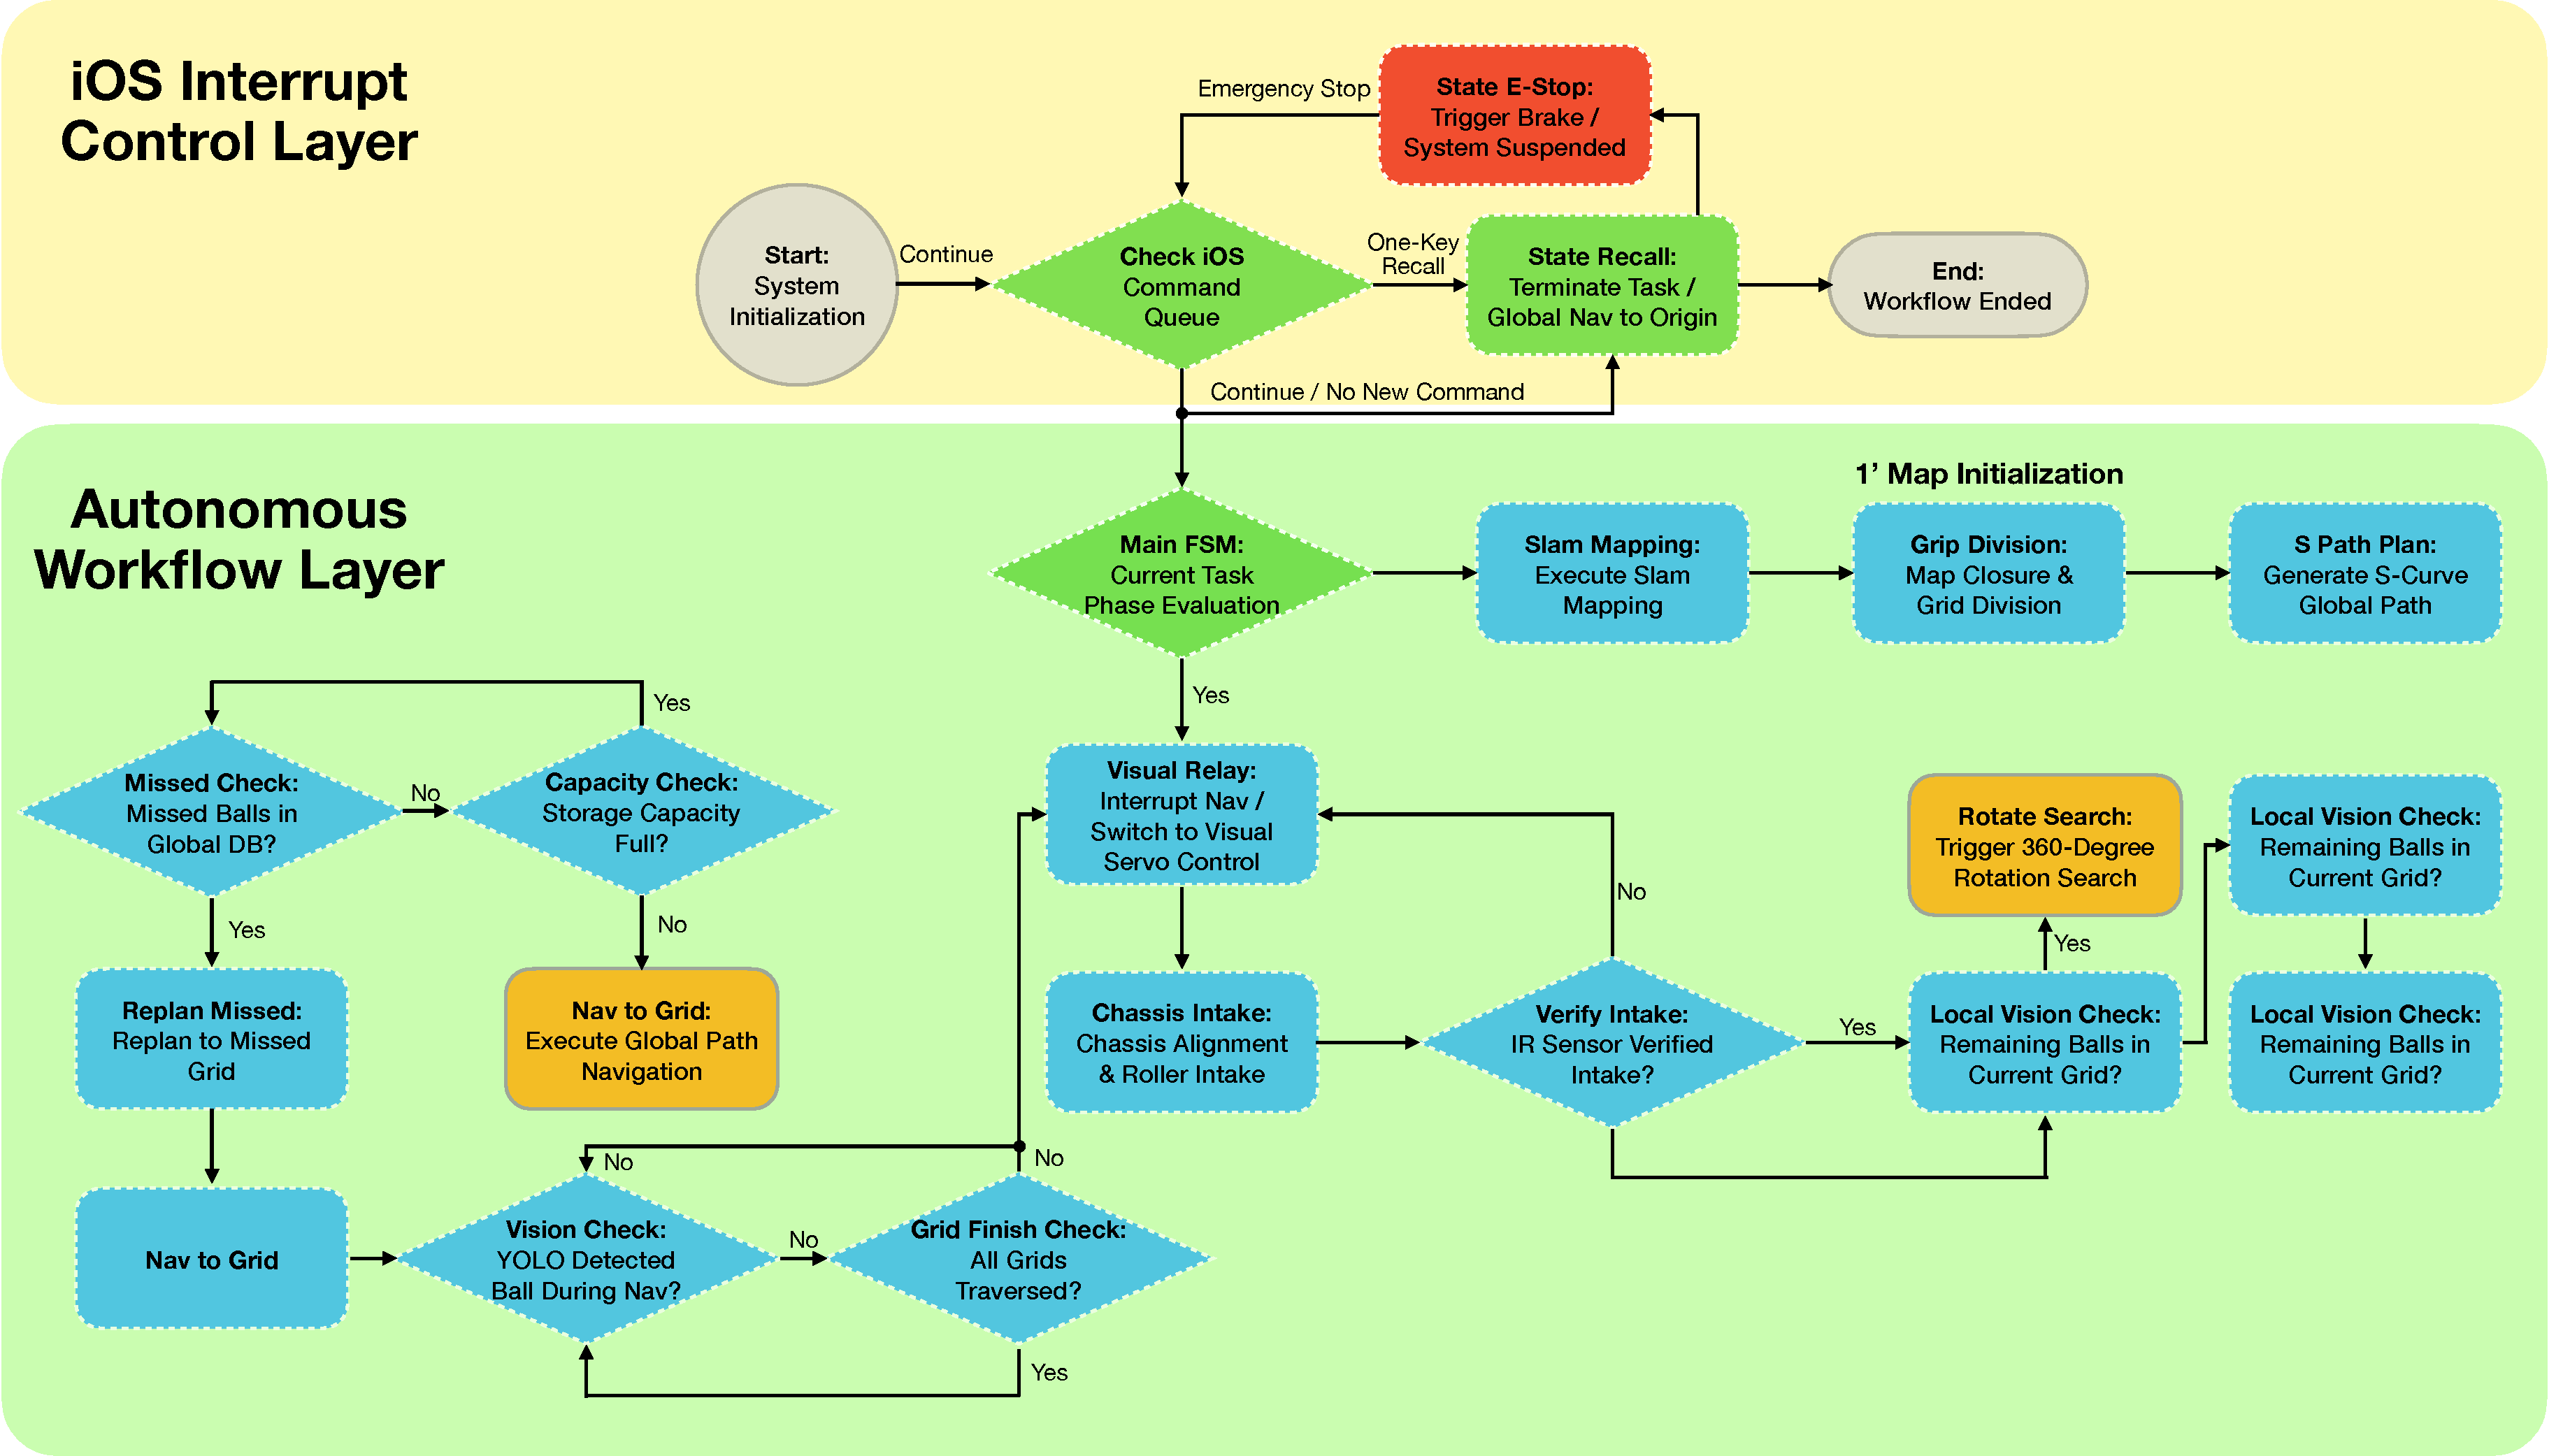
\includegraphics[width=0.92\linewidth]{figures/fig_workflow.pdf}
  \caption{Hierarchical FSM flow diagram. The upper interrupt control layer preempts the lower autonomous workflow at any time. The autonomous layer progresses through three phases: mapping, waypoint navigation, and visual closed-loop retrieval with 360\textdegree{} post-ingestion sector sweep.}
  \label{fig:workflow}
\end{figure}

\subsubsection{iOS Interrupt Control Layer (Upper FSM)}

The upper FSM continuously polls the iOS command queue over UDP. Two high-priority interrupt commands preempt any ongoing autonomous behavior:

\begin{enumerate}
  \item \textbf{Emergency Stop (E-STOP):} Immediately engages chassis braking and suspends all autonomous logic until the operator issues a resume command.
  \item \textbf{One-Touch Recall:} Terminates the current mission and invokes the Nav2 planner to navigate the robot to the predefined origin pose.
\end{enumerate}

\subsubsection{Autonomous Workflow Layer (Lower FSM)}

The lower FSM transitions through three sequential mission phases:

\textbf{Phase 1 --- Mapping \& Global Planning.}
SLAM toolbox constructs the occupancy grid while the operator teleoperates the robot around the court perimeter. Once the map is saved, an S-shaped waypoint sequence is loaded into the Nav2 waypoint follower.

\textbf{Phase 2 --- Waypoint Navigation \& Interrupt Handling.}
Before dispatching each waypoint, two pre-navigation checks execute: a missed-ball database lookup for previously detected but unrecovered ball locations, and a storage capacity check that triggers recall if the onboard bay is full. If clear, Nav2 navigates to the next waypoint. During traversal, the YOLO pipeline runs concurrently; upon detection, navigation is interrupted and Phase~3 activates. When all waypoints are visited, the system triggers a recall.

\textbf{Phase 3 --- Visual Closed-Loop Retrieval.}
This phase is implemented in \texttt{chassis\_ctrl.py} as an implicit state machine driven by three Boolean flags defined at module level:

\begin{minted}{python}
visual_error_x = 0
target_locked  = False    # whether a ball is currently locked
scan_needed    = False    # whether to perform a 360-degree scan
no_ball_counter = 0       # consecutive frames without detection
\end{minted}

The main control loop transitions between behavioral modes based on these flags and the real-time IR distance sensor reading (millimetres). The transition logic at the top of the loop is:

\begin{minted}{python}
target_valid = vn.target_locked
need_scan    = vn.scan_needed
dist = ds.latest_distance if ds.latest_distance is not None else 8848

if target_valid:
    is_chasing_sequence = True
    last_valid_dist = dist
elif need_scan:
    is_chasing_sequence = False
    last_valid_dist = 8848
\end{minted}

When \texttt{is\_chasing\_sequence} is active, the controller executes three priority-ordered behaviors based on the current sensor reading. Key numerical thresholds are listed in Table~\ref{tab:fsm_params}.

\begin{table}[!htb]
  \footnotesize
  \centering
  \caption{FSM Phase 3 operational parameters implemented in \texttt{chassis\_ctrl.py} and \texttt{video\_node.py}.}
  \label{tab:fsm_params}
  \begin{tabular}{@{}lll@{}}
    \toprule
    \textbf{Stage} & \textbf{Parameter} & \textbf{Value} \\
    \midrule
    Target acquisition & Consecutive no-ball frames to trigger scan & 15 \\
    Visual servoing & Turn PID (\texttt{pid\_turn}) & $K_p=0.15, K_i=0.03, K_d=0.03$ \\
                       & Turn PID output limits & $[-50, 50]$ \\
                       & Forward PID (\texttt{pid\_forward}) & $K_p=0.5, K_i=0.1, K_d=0.05$ \\
                       & Forward PID output limits & $[-40, 40]$ \\
                       & Alignment-priority threshold & $\lvert\text{error\_x}\rvert > 40$\,px \\
                       & Open-loop cruise speed & 30 (forward) \\
    Blind-zone relay & Target-lost distance guard & $\text{dist} < 450$\,mm \\
                       & Last-valid proximity guard & $\text{last\_valid\_dist} < 300$\,mm \\
    Ingestion trigger & Pre-spin distance threshold & $\leq 200$\,mm \\
                       & Motor pre-spin duty & 90 ($\sim$35\%) \\
                       & Approach speed during ingestion & 30 (forward) \\
    Ingestion confirm & Disappearance distance threshold & $> 250$\,mm \\
                       & Consecutive disappearance frames & 10 (200\,ms) \\
                       & Hard timeout & 3.0\,s \\
    360\textdegree{} sector sweep & In-place rotation speed & 30 (turn) \\
    \bottomrule
  \end{tabular}
\end{table}

After confirmed ingestion, the robot executes a $360^\circ$ in-place rotational scan. If YOLO detects another ball during the scan, the chasing sequence re-engages (looping back to visual servoing). If the scan completes with no detections, the sector is marked as cleared, the global ball-coordinate database is updated, and control returns to the main FSM for the next waypoint dispatch. The detailed implementation of the reactive control pipeline is presented in Section~\ref{sec:detailed_software}.


\subsection{Class Design}
\label{sec:class-design}

\paragraph{CourtNavigationManager Class Description}

The central orchestrator of the autonomous workflow is the \texttt{CourtNavigationManager} class, which bridges the ROS2 navigation stack, the computer vision pipeline, and the hardware actuation interfaces through the hierarchical FSM. At the implementation level, the Phase~3 reactive FSM logic resides in \texttt{chassis\_ctrl.py} using the Boolean flag mechanism described above; \texttt{CourtNavigationManager} coordinates the higher-level phase transitions and Nav2 dispatch.

\begin{table}[H]
  \footnotesize
  \centering
  \renewcommand{\arraystretch}{1.3}
  \begin{tabularx}{\linewidth}{|l|X|}
    \hline
    \rowcolor[RGB]{220,220,220} \textbf{Attribute} & \textbf{Description} \\ \hline
    Class Name & \texttt{CourtNavigationManager} \\ \hline
    Aggregated Classes & \texttt{YoloDetector}, \texttt{Nav2PlannerClient}, \texttt{DjiChassisController}, \texttt{MotorPwmDriver}, \texttt{IrSensorReader} \\ \hline
    Associated Classes & \texttt{MjpegStreamServer}, \texttt{IosCommandReceiver} (UDP listener for iOS interrupts) \\ \hline
    Data Members &
    \textbullet~ \texttt{master\_state}: Enum (\texttt{MAPPING}, \texttt{NAVIGATING}, \texttt{INTERCEPTING}, \texttt{RETRIEVING}, \texttt{RECALLING}, \texttt{E\_STOP}). \newline
    \textbullet~ \texttt{robot\_pose\_global}: Pose $(x, y, \theta)$ obtained from Nav2 AMCL localization. \newline
    \textbullet~ \texttt{waypoint\_queue}: Ordered S-shaped sequence of navigation goals. \newline
    \textbullet~ \texttt{missed\_ball\_db}: List of $(x, y)$ coordinates of detected but unrecovered balls. \newline
    \textbullet~ \texttt{storage\_capacity}: Current ball count in the onboard bay. \\ \hline
    Member Functions &
    \textbullet~ \texttt{process\_ios\_interrupt()}: Receives UDP commands from the iOS app (E-STOP / Recall / Continue). \newline
    \textbullet~ \texttt{update\_master\_state()}: High-level FSM transitions based on vision events, waypoint progress, and capacity thresholds. \newline
    \textbullet~ \texttt{generate\_coverage\_path()}: Generates S-shaped waypoint sequence from the SLAM map. \newline
    \textbullet~ \texttt{dispatch\_nav2\_goal()}: Sends a target pose to Nav2 and monitors execution. \newline
    \textbullet~ \texttt{handle\_visual\_intercept()}: Suspends Nav2, switches to PD visual servoing, triggers intake on proximity confirmation. \newline
    \textbullet~ \texttt{perform\_360\_scan()}: In-place rotation with YOLO monitoring; loops back to retrieval if a new ball is found. \\ \hline
    Processing & Operates in a dedicated high-priority thread. Fuses Nav2 pose with YOLO detections, executes the hierarchical FSM, dispatches velocity commands, and manages motor triggering. \\ \hline
  \end{tabularx}
\end{table}
